\documentclass[aspectratio=169]{beamer}
\usepackage{hyperref}
\hypersetup{
	pdfstartpage=1 ,
	pdfpagemode=FullScreen % Start in full-screen mode
	% Ensure it starts from page 1
}
\usetheme{CambridgeUS}
\usecolortheme{beaver}
\useoutertheme[subsection=false]{smoothbars}
\usepackage{graphicx}
\usepackage{dirtytalk}
\usepackage{pgf}
\graphicspath{{img}}
\usepackage{siunitx}
\usepackage{multicol}
\usepackage{multimedia}
\usepackage{minted}
\usepackage{subcaption}
\usepackage{braket}
\setcounter{MaxMatrixCols}{11}


\setminted{fontsize=\scriptsize, tabsize=2}

\captionsetup{font=footnotesize}

\newcounter{framenumberbeforeappendix}


\input{package/beamercolorthemebeaver.sty}

%\input{beamercolorthemespruce.sty}

\title[QA-Prolog]{High level programming language for quantum computing}
\author{Davide Camino}
\date{\texttt{davide.camino@edu.unito.it}}
\institute[UniTO]{\includegraphics[width=.15\linewidth]{logo_col}}


\begin{document}

\part{Main}
\begin{frame}[plain]
	\transfade[duration=0.5]
	\maketitle
\end{frame}


\begin{frame}{Obbiettivo del lavoro}
	\begin{center}
		\begin{minipage}{.7\linewidth}
			\hfill
			\begin{block}{}
				\centering
				\large
				\textbf{Reasoning su quantum computer}
			\end{block}
			\hfill
			\begin{block}{}
				\centering
				Base di conoscenza classica + query
			\end{block}
			\hfill
			\begin{block}{}
				\centering
				Embedding su quantum computer
			\end{block}
			\hfill
			\begin{block}{}
				\centering
				Esecuzione e recupero risultati
			\end{block}
			\hfill
		\end{minipage}
	\end{center}
\end{frame}
\section{QA-Prolog}
\begin{frame}{QA-Prolog}
	
\end{frame}
\begin{frame}{Pipeline}
	
\end{frame}
\begin{frame}{QMASM}
	
\end{frame}
\begin{frame}{QMASM}{Esempio}
	
\end{frame}
\begin{frame}{Yosys - edif2qmasm}
	
\end{frame}
\begin{frame}{Yosys - edif2qmasm}{Esempio}
	
\end{frame}
\begin{frame}{QA-Prolog}
	
\end{frame}
\begin{frame}{QA-Prolog}{Esempio}
	
\end{frame}

\section{AQC \& QAOA}
\begin{frame}{Non un solo paradigma}
	\begin{center}
		\begin{minipage}{.6\linewidth}
			\begin{block}{}
				\centering
				Problema QUBO/Ising
				\vspace{-.3cm}
				\[
				\mathcal{H}_f
				\]
			\end{block}
		\end{minipage}
	\end{center}
	\begin{figure}[h]
		\centering
		\begin{subfigure}{0.3\linewidth}
			\centering
			\includegraphics[width=\linewidth]{simulate_annealing}
			\caption{Simulated annealing (Li Yang)}
		\end{subfigure}
		\hfill
		\begin{subfigure}{0.3\linewidth}
			\centering
			\includegraphics[width=\linewidth]{QA}
			\caption{Quantum annealing (K. Chakrabarti, A. Das)}
		\end{subfigure}
		\hfill
		\begin{subfigure}{0.3\linewidth}
			\centering
			\includegraphics[width=\linewidth]{QAOA_sketch}
			\caption{QAOA (Z. Zhou, Y. Du, X. Tian, D. Tao)}
		\end{subfigure}
		\caption{Single rappresenbtation 3 different approaches}
	\end{figure}
\end{frame}

\section{Esempio Completo}
\begin{frame}[fragile]{Esempio completo}{Quantum Simpson}
	\begin{figure}
        \begin{minipage}{.9\linewidth}
            \hrule
            \begin{minted}{xml}

<owl:NamedIndividual rdf:about="http://www.people#marge">
    <rdf:type rdf:resource="http://www.people#People"/>
    <www:marry rdf:resource="http://www.people#homer"/>
    <www:parent_of rdf:resource="http://www.people#bart"/>
</owl:NamedIndividual>
            \end{minted}
            \hrule
        \end{minipage}
        \caption{Marge Simpson entry}
    \end{figure}
    \vspace{-.3cm}
    \begin{figure}
        \includegraphics[width=.55\linewidth]{people.pdf}
        \caption{Ontology Structure}
    \end{figure}
\end{frame}


\begin{frame}[fragile]{Da OWL-rdf a Prolog}
	\begin{minipage}{.35\linewidth}
		\begin{figure}
			\begin{minipage}{.95\linewidth}
				\hrule
				\begin{minted}{Prolog}

person(marge).
person(bart).
person(jackie).
person(selma).
person(ling).

parent_of(marge, bart).
parent_of(jackie, marge).
parent_of(jackie, selma).
parent_of(selma, ling).

son_of(P, Q) :- parent_of(Q, P).

gran_parent_of(P, Q) :-
	son_of(Q, X),
	son_of(X, P).
				\end{minted}
				\hrule
                \caption{Prolog Ontology}
			\end{minipage}
		\end{figure}
	\end{minipage}
	\hfill
	\begin{minipage}{.62\linewidth}
        \begin{block}{Interrogazione}
			\begin{center}
				\scriptsize \texttt{QA-Prolog --verbose --qmasm-args="--solver=sim\_anneal --postproc=opt" --query='gran\_parent\_of(P1, P2).' family.pl}
			\end{center}
		\end{block}
		\begin{figure}
			\begin{minipage}{.4\linewidth}
				\hrule
				\begin{minted}{text}

P1 = jackie
P2 = bart

P1 = jackie
P2 = selma
				\end{minted}
				\hrule
			\end{minipage}
			\caption{Query Result 1}
		\end{figure}
        \vspace{-.5cm}
        \begin{figure}
			\begin{minipage}{.4\linewidth}
				\hrule
				\begin{minted}{text}

P1 = jackie
P2 = bart
				\end{minted}
				\hrule
			\end{minipage}
			\caption{Query Result 2}
		\end{figure}
	\end{minipage}
\end{frame}

\begin{frame}[fragile]{Limitazioni del simulatore}
	\begin{minipage}{.35\linewidth}
		\begin{figure}
			\begin{minipage}{.95\linewidth}
				\hrule
				\begin{minted}{Prolog}

cousins(P, Q):-
	gran_parent_of(X, P),
	gran_parent_of(X, Q),
	parent_of(Y, P),
	parent_of(Z, Q),
	Z \= Y.
				\end{minted}
				\hrule
                \caption{Cousins rule}
			\end{minipage}
		\end{figure}
	\end{minipage}
	\hfill
	\begin{minipage}{.62\linewidth}
        \begin{block}{Interrogazione}
			\begin{center}
				\scriptsize \texttt{QA-Prolog --verbose --qmasm-args="--solver=sim\_anneal --postproc=opt" --query='cousins(P1, P2).' family.pl}
			\end{center}
		\end{block}
		\begin{figure}
			\begin{minipage}{.55\linewidth}
				\hrule
				\begin{minted}{text}

QA-Prolog: No solutions were found
				\end{minted}
				\hrule
			\end{minipage}
			\caption{Query Result}
		\end{figure}
	\end{minipage}
\end{frame}
\section{Lavoro Futuro}
\begin{frame}{Lavoro Futuro}
    \begin{minipage}{.48\linewidth}
        \begin{block}{Monte}
            \begin{itemize}
                \item Compilatore OWL/RDF $\rightarrow$ Prolog
                \item Sperimentare altri linguaggi
            \end{itemize}
        \end{block}
    \end{minipage}
    \hfill
    \begin{minipage}{.48\linewidth}
        \begin{block}{Valle}
            \begin{itemize}
                \item Aggiungere simulated annealing
                \item Interfacciare QMASM con quantum gate
            \end{itemize}
        \end{block}
    \end{minipage}
    \vspace{.5cm}
    \begin{center}
        \begin{minipage}{.7\linewidth}
            \begin{block}{}
                    \begin{itemize}
                        \item Mantenere aggiornati i componenti
                        \item Testare su hardware quantistico
                        \item Confronto ACQ e QAOA
                    \end{itemize}
            \end{block}
        \end{minipage}
    \end{center}
\end{frame}

\part{Ringraziamenti}
\begin{frame}[plain]
	\vspace{1cm}
	\begin{center}
		{
			\Huge
			Grazie per l'attenzione
		}
		
		\vspace{.5cm}
		Davide Camino
		
		\vspace{.1cm}
		{\small \texttt{davide.camino@edu.unito.it}}
		
		\vspace{.5cm}
		\includegraphics[width=.15\linewidth]{logo_col}
	\end{center}
\end{frame}
\setcounter{framenumberbeforeappendix}{\value{framenumber}}
\part{Materiale aggiuntivo}
\section{Quantum Computing}


\begin{frame}{Perché il quantum computing}
	\begin{minipage}{\linewidth}
		\begin{minipage}{.48\linewidth}
			\begin{block}{Grazie a}
				\begin{itemize}
					\item Entanglement
					\item Superposition
				\end{itemize}
			\end{block}
		\end{minipage}
		\hfill
		\begin{minipage}{.48\linewidth}
			immagine
		\end{minipage}
	\end{minipage}
	\begin{minipage}{\linewidth}
		\begin{minipage}{.48\linewidth}
			\begin{block}{Violiamo}
				Strong Church-Turing Thesis
			\end{block}
		\end{minipage}
		\hfill
		\begin{minipage}{.48\linewidth}
			immagine
		\end{minipage}
	\end{minipage}
\end{frame}


\begin{frame}{Due paradigmi di programmazione}
	\begin{minipage}{\linewidth}
		\begin{minipage}{.48\linewidth}
			\begin{block}{}
				Quantum Gate
			\end{block}
		\end{minipage}
		\hfill
		\begin{minipage}{.48\linewidth}
			\begin{block}{}
				Quantum Annealing
			\end{block}
		\end{minipage}
	\end{minipage}
	\begin{minipage}{\linewidth}
		\begin{minipage}{.48\linewidth}
			immagine
		\end{minipage}
		\hfill
		\begin{minipage}{.48\linewidth}
			immagine
		\end{minipage}
	\end{minipage}
\end{frame}


\begin{frame}{Quantum Gate}
	\begin{minipage}{.48\linewidth}
		\begin{block}{}
			\begin{itemize}
				\item Formalismo molto studiato
				\item Gate Reversibili
				\item  Set di porte universali
				\item  Algoritmi di Shore, ecc.
			\end{itemize}
		\end{block}
	\end{minipage}
	\hfill
	\begin{minipage}{.48\linewidth}
		immagine
	\end{minipage}
\end{frame}


\begin{frame}{Quantum Annealer}
	\begin{minipage}{.48\linewidth}
		immagine
	\end{minipage}
	\hfill
	\begin{minipage}{.48\linewidth}
		\begin{block}{}
			\begin{itemize}
				\item Ispirato a Simulated Annealling
				\item Effetto tunneling
				\item Adiabatic Quantum Computing (AQC)
				\item $\mathcal{H}(t) =s(t) \mathcal{H}_i + (i-s(t)) \mathcal{H}_f $
			\end{itemize}
		\end{block}
	\end{minipage}	
\end{frame}
\input{chapter/appendix/QA-prolog}
\section{AQC \& QAOA}
\begin{frame}{Non un solo paradigma}
	\begin{center}
		\begin{minipage}{.6\linewidth}
			\begin{block}{}
				\centering
				Problema QUBO/Ising
				\vspace{-.3cm}
				\[
				\mathcal{H}_f
				\]
			\end{block}
		\end{minipage}
	\end{center}
	\begin{figure}[h]
		\centering
		\begin{subfigure}{0.3\linewidth}
			\centering
			\includegraphics[width=\linewidth]{simulate_annealing}
			\caption{Simulated annealing (Li Yang)}
		\end{subfigure}
		\hfill
		\begin{subfigure}{0.3\linewidth}
			\centering
			\includegraphics[width=\linewidth]{QA}
			\caption{Quantum annealing (K. Chakrabarti, A. Das)}
		\end{subfigure}
		\hfill
		\begin{subfigure}{0.3\linewidth}
			\centering
			\includegraphics[width=\linewidth]{QAOA_sketch}
			\caption{QAOA (Z. Zhou, Y. Du, X. Tian, D. Tao)}
		\end{subfigure}
		\caption{Single rappresenbtation 3 different approaches}
	\end{figure}
\end{frame}

\section{Ontologie}
\begin{frame}{Ontologie}
	\begin{minipage}{.48\linewidth}
        \begin{block}{Cos'è un'ontologia}
            \begin{itemize}
                \item Insieme di fatti
                \item Riguardanti un dominio di interesse
                \item Prevengono interpretazioni sbagliate
                \item Assicurano la cooperazione tra software
            \end{itemize}
        \end{block}
        \begin{block}{Come si definisce un'ontologia}
            \begin{itemize}
                \item Ontology Web Language (OWL)
                \item Diversi \say{flavours}
                \begin{itemize}
                    \item OWL Full
                    \item OWL DL
                \end{itemize}
                \item Classi Individui e Relazioni
            \end{itemize}
        \end{block}
    \end{minipage}
    \hfill
    \begin{minipage}{.48\linewidth}
        \begin{figure}[h]
            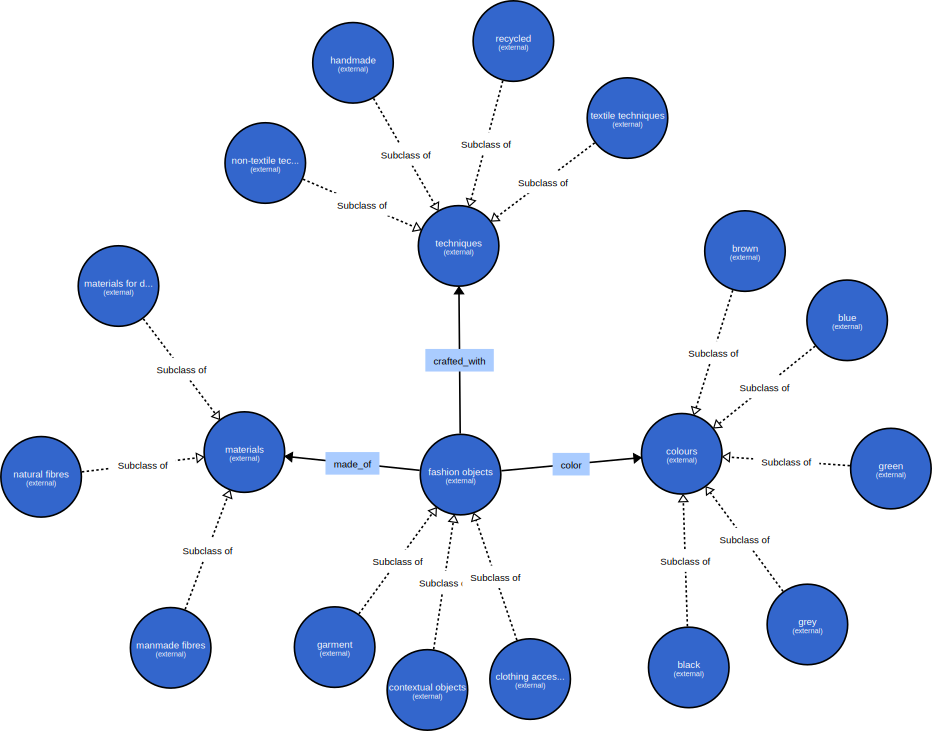
\includegraphics[width=\linewidth]{europeana_relation.pdf}
        \end{figure}
    \end{minipage}
\end{frame}

\begin{frame}{Inferenze in OWL}
	\begin{minipage}{.48\linewidth}
        \begin{block}{Complessità}
            \begin{itemize}
                \item Variazione sintattica di $\mathcal{SROIQ}$
                \item $\mathcal{ALC}$ è una restrizione di $\mathcal{SROIQ}$
                \item $\mathcal{ALC}$ è PSpace-hard
            \end{itemize}
        \end{block}
        \begin{block}{Reasoner}
            \begin{itemize}
                \item Pellet
                \item Fact++
                \item HermiT
                \item \dots
            \end{itemize}
        \end{block}
    \end{minipage}
    \hfill
    \begin{minipage}{.48\linewidth}
        \begin{figure}[h]
            \includegraphics[width=.8\linewidth]{Complexity.pdf}
        \end{figure}
    \end{minipage}
\end{frame}

\setcounter{framenumber}{\value{framenumberbeforeappendix}}

\end{document}
